\section{Определение и характеристика}

\begin{frame}{Определение}
	\begin{columns}
		\begin{column}{.5\textwidth}
			\begin{definition}{Определение}
				Тестирование производительности -- набор мер по изучению и анализу производительности системы, т.е. потребления вычислительных ресурсов.
			\end{definition}
		\end{column}
		\begin{column}{.5\textwidth}
			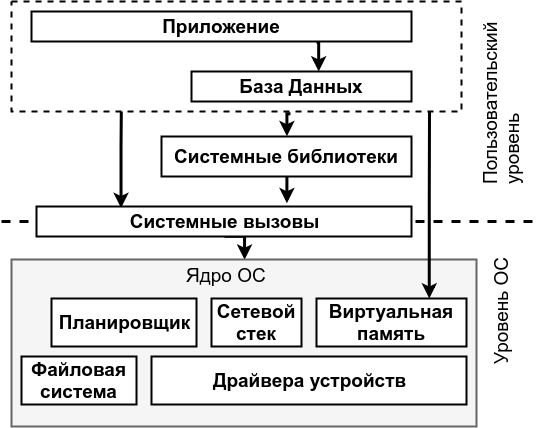
\includegraphics[width=\textwidth]{img/system_stack.png}
		\end{column}
	\end{columns}
\end{frame}

\begin{frame}{Что можно измерять?}
	\begin{description}
		\item[\textbf{Задержка (latency)}] -- время, которое ожидает операция для того чтобы быть выполненной.
		\item[\textbf{Степень использования (utilization)}] -- мера занятости ресурса, например, загрузка ЦП или объем занимаемой ОП.
		\item[\textbf{Операции ввода-вывода в секунду (IOPS)}] -- скорость работы приложений с периферийными устройствами, например, жесткими дисками.
		\item[\textbf{Пропускная способность (throughput)}]  -- количество каких-либо операций в секунду (запросов, обработанных байтов).
	\end{description}
\end{frame}

\begin{frame}{Зачем и как измерять?}
	\begin{columns}
		\begin{column}{.5\textwidth}
				\begin{block}{Локализовать и устранить недостатки}
					\begin{itemize}
						\item Профилирование
						\begin{itemize}
							\item gprof -- простой во всех смыслах
							\item Intel VTune -- дорого-богато
							\item perf tools -- швейцарский нож для профилирования
							\item Valgring -- слишком тяжелый
						\end{itemize}
						\item Макробенчмаркинг
						\begin{itemize}
							\item time -- (а почему нет-то?)
							\item iostat -- IOPS блочных устройств
							\item iperf -- производительность сети
						\end{itemize}
					\end{itemize}
				\end{block}
		\end{column}
		\begin{column}{.5\textwidth}
			\begin{block}{Сравнение кода между собой}
				\begin{itemize}
					\item Микробенчмаркинг (С++)
					\begin{itemize}
						\item Google Benchmark -- большая и функциональная библиотека
						\item Hayai -- маленький и простой заголовочник
						\item x86 rdtsc и chrono -- собери бенчмарк сам (сложность зависит от целей)
					\end{itemize}
				\end{itemize}
			\end{block}
		\end{column}
	\end{columns}
\end{frame}

\begin{frame}{Методики измерения?}
	\begin{columns}
		\begin{column}{.5\textwidth}
			\textbf{Тысячи их:}
			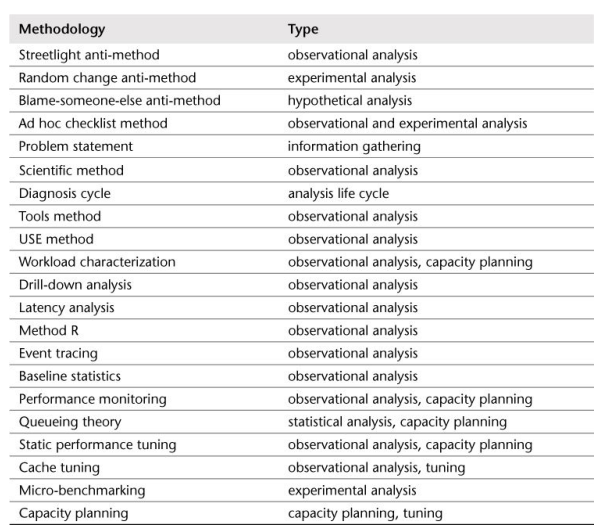
\includegraphics[width=\textwidth]{img/methodology.png}
		\end{column}
		\begin{column}{.5\textwidth}
			Что важнее: \textbf{как делать не надо!}
			\begin{itemize}
				\item Поиск только при свете дня (фонаря) -- не надо искать очевидное.
				\item Тестирование вслепую
				\item Виноват не я! Не надо искать причину в других людях, а не в коде.
			\end{itemize}
		\end{column}
	\end{columns}

\end{frame}

\begin{frame}{Что мешает?}
	\begin{itemize}
		\item \textbf{СУБЪЕКТИВНОСТЬ И ПОГРЕШНОСТЬ}
		\item Процессор
		\begin{itemize}
			\item Кэш (он вообще везде мешает)
			\item Конвейер
			\item Многоядерность
			\item Эвристики (branch prediction)
		\end{itemize}
		\item Компилятор и его оптимизации
	\end{itemize}
	\begin{center}
		\textbf{Как это решается?}
	\end{center}
	\begin{itemize}
		\item Итеративное выполнение (для бенчмаркинга)
		\item Закон больших чисел и статистика
		\item Фиксация процесса на ядре, установка одного режима работы ЦП(!)
		\item Принуждение компилятора (хитростью и напрямую)
	\end{itemize}
\end{frame}